%%%%%%%%%%%%%%%%%%%%%%%%%%%%%%%%%%%%%%%%%%%%%%%%%%%%%%%%%%%%%%%%%%%%%%%%%%%%%%%%
%%%%%%%%%%%%%%%%%%%%%%%%%%%%%%%%%%%%%%%%%%%%%%%%%%%%%%%%%%%%%%%%%%%%%%%%%%%%%%%%
\subsection{Multiple Contacts}
Multiple abstract models can be strung together to model falling with
a sequence of contacts. Each abstract model describes the motion from
the impact moment $\hat{t}_i$ to the next impact moment
$\hat{t}_{i+1}$. The first abstract model is initialized by the
initial states of COM and COP of the robot at the beginning of the
fall. As the current stopper hits the ground, a new abstract
model is initialized: the COM of the current pendulum at $\hat{t}_{i+1}$ becomes the
initial COM of the new abstract model and the tip of the current
stopper becomes the pivot of the new abstract model. Using multiple
abstract models to represent the falling motion, our goal is to search
for a sequence of contacts whose maximum vertical impulse is
minimized.

Before we formulate the search problem formally, it is important to
note that the number of contacts used to break a fall, in theory, can
be arbitrarily large. In the limit, if a robot could morph into a
rolling ball without slipping, the number of contacts would be infinite and
the vertical impulse of the fall would be zero (the initial momentum is never
dissipated). In practice, however, the robot has only a limited number
of preferred contact points, such as feet, knees, or
hands. Furthermore, these contact points can only be applied in
certain sequences due to the hardware design and kinematic
constraints. 

\begin{figure}[ht]
\center
  %% 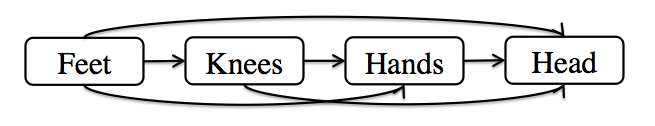
\includegraphics[width=3.0in]{images/contact_graph.png}
  %% 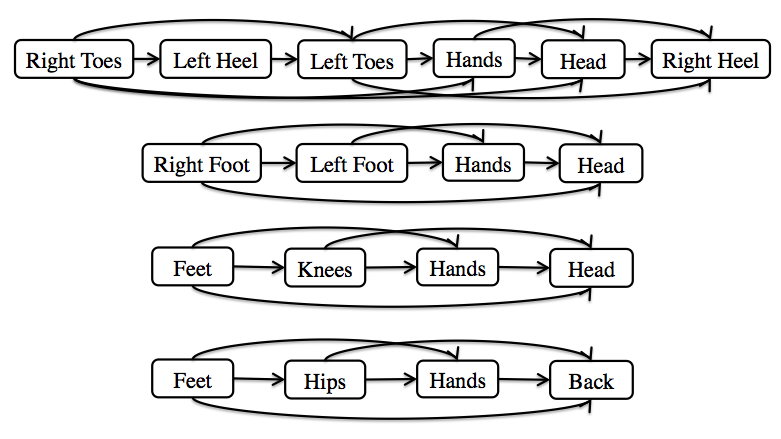
\includegraphics[width=3.0in]{images/four_contact_graphs.png}
  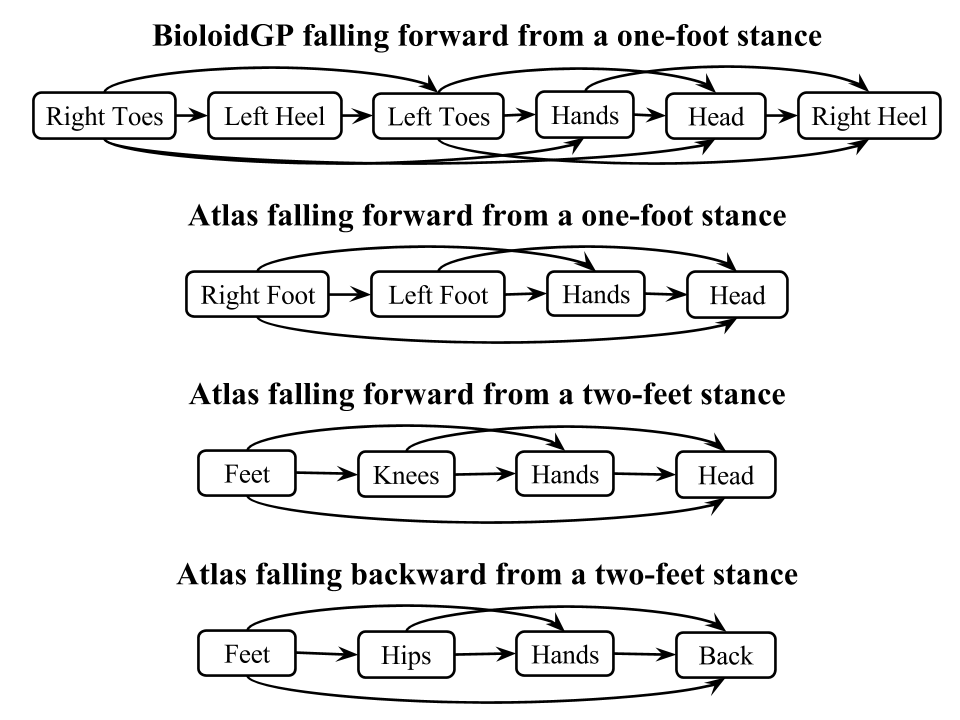
\includegraphics[width=0.8\textwidth]{images/all_contact_graphs.png}
  \caption{Contact graphs}
  \label{fig:falling_contact_graph}
\end{figure}

Utilizing these constraints, we introduce a data structure, called a
\emph{contact graph}, to narrow down the search space to only those
contact sequences achievable by a given robot. A contact graph is a
directed graph $G(V_{c}, E_{c})$ which vertices are the preferred
contact points on the robot. If there exists an edge from node $c_1$
to node $c_2$, it indicates that $c_2$ is a valid subsequent contact
point to $c_1$. Given a robot, we can design a contact graph to
represent all possible falling strategies the robot can employ. For
example, a path from feet to knees to hands in \figref{falling_contact_graph}
represents the falling strategy described in \cite{Fujiwara:2002:UFM}.

%%%%%%%%%%%%%%%%%%%%%%%%%%%%%%%%%%%%%%%%%%%%%%%%%%%%%%%%%%%%%%%%%%%%%%%%%%%%%%%%
\paragraph{Plan for contact sequence}
With the contact graph and the initial state of the robot as input, we
now describe our algorithm that searches for an optimal sequence of
contacts using multiple abstract models. 

We formulate the problem as a Markov Decision Process, a framework for
modeling decision making with a long-term cost. We define a state at
each impact moment as
$\vc{x} = \{c_1, \hat{t},\theta_1, r_1, \dot{\theta}_1, \dot{r}_1\}
\in \mathcal{X}$,
where $c_1$ denotes the contact point on the robot, $\hat{t}$ denotes
the time when the impact occurs, and other parameters describe the
position and the velocity of the pendulum at the impact moment. An
action
$\vc{a}=\{c_2, \theta_2, \Delta t, \dot{r}^d_1\} \in \mathcal{A}$
describes the contact point on the robot used as the stopper ($c_2$),
the position of the stopper at the next impact moment ($\theta_2$),
the elapse time from the previous impact moment to the next impact
moment ($\Delta t$), and the desired speed of the pendulum length
during the current contact ($\dot{r}^d_1$). Note that the length of
the stopper $r_2$ at the next impact moment can be derived from $r_1$,
$\theta_1$, and $\theta_2$ by calculating the intersection of the
stopper and the ground.

% The action space is
% defined as $\vc{a}=\{c_2, \dot{r}^d_1, \theta_2, t\} \in \mathcal{A}$
% which comprises the contact point used as the tip of the stopper
% $c_2$, the desired rod velocity $\dot{r}^d_1$, the angle between the
% pendulum rod and the stopper rod $\theta_2$ when it hits the ground,
% and the time $t$ when the stopper hits the ground. Note that the length
% of the stopper $r_2$ at the activation time can be reconstructed from
% $r_1$, $\theta_1$, and $\theta_2$ by calculating the intersection of
% the stopper and the ground.

%% \begin{figure}[ht]
%%   \center
%%   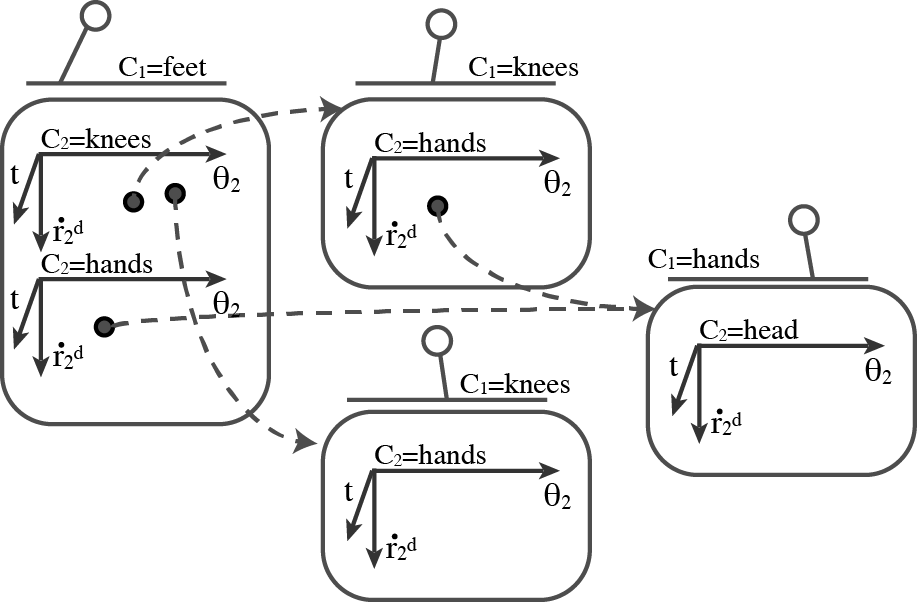
\includegraphics[width=3.2in]{images/recursive.png}
%%   \caption{\updated{We illustrate the concept of the
%%       recursive search by visualizing the states of pendulums (small drawings on boxes)
%%       and possible actions (4D tables in boxes).
%%       Note that different actions can possibley result the same state. }}
%%   \label{fig:falling_recursion}
%% \end{figure}

Our goal is to search for the best action sequence in $\mathcal{A}$ to
minimize the maximum impulse. The long-term cost of an action $\vc{a}$
taken at a state $\vc{x}$ can be expressed as
\begin{equation}
\max\big(g(\vc{x}, \vc{a}), v(f(\vc{x}, \vc{a}))\big),
\label{eq:falling_actionEval}
\end{equation}
where $g(\vc{x}, \vc{a})$ is the local cost function which computes
the vertical impulse due to the action $\vc{a}$ taken at the state
$\vc{x}$, $f(\vc{x}, \vc{a})$ is the transition function which outputs
the state after taking $\vc{a}$ at $\vc{x}$, and $v(\vc{x})$ is
the $cost \mhyphen to \mhyphen go$ function that yields the minimal impulse starting from
$\vc{x}$ following the best actions. The cost-to-go function can be
expressed recursively as
\begin{equation}
v(\vc{x}) = \min_{\vc{a}} \max(g(\vc{x}, \vc{a}), v(f(\vc{x}, \vc{a}))).
\label{eq:falling_cost-to-go}
\end{equation}
Determining the best action from a given state is a 4D search
problem. Every evaluation of an action (\eqnref{falling_actionEval}) invokes a
cost-to-go function (\eqnref{falling_cost-to-go}), which recursively generates
another 4D search problem. Although the recursive
search exponentially expands with the number of contacts, the state
space we need to consider is quite limited due to the monotonicity
nature of falling motion. That is, as the robot falls, $\theta_1$
changes monotonically from the initial value to $0$ (or
$\pi$). Likewise, $\dot{\theta}_1$ will never exceed the range between
the initial velocity and $0$. As a result, the algorithm visits a
large number of repeated states during the search. We exploit this
property using dynamic programming with k-nearest neighbor algorithm
to significantly expedite the search (details later).

\begin{algorithm}
  \If {$\dot{\theta}_1<0$} {
    \Return $0$\; 
    \label{alg:line:falling_terminal}
  }
  \If {kNN has $\vc{x}$}
      { \label{alg:line:falling_knn_query} 
        \Return $kNN[\vc{x}]$\;
      }
      $\bar{j} = \infty$\;
      \For {$\dot{r}_1^d \in \mathcal{V}$} { \label{alg:line:falling_rdot}
        $\vc{x}^{now}=\vc{x}$\;
        $\Delta t=0$\;
        \While {$\theta_1^{now} < \pi/2$} { \label{alg:line:falling_theta}
          $\mathcal{S} = generate\_stoppers(\vc{x}^{now}, \Delta t)$\; \label{alg:line:falling_collect}
          \For {$c_2, \theta_2 \in \mathcal{S}$} {
            $\vc{a}=\{(c_2, \theta_2, \Delta t, \dot{r}_1^d)\}$\;
            $\vc{x}^{+}=f(\vc{x}^{now}, \vc{a}$)\;
            $ j^{+}=g(\vc{x}^{now}, \vc{a}$)\;
            $j^{*}$ = $cost \mhyphen to \mhyphen go(\vc{x}^{+})$\;
            $\bar{j}$ = $\min(\bar{j}, \max{(j^{+}, j^{*})})$\;
          }
          $\vc{x}^{now}$ = $simulate\_pendulum(\vc{x}^{now}, \dot{r}_1^d$)\; \label{alg:line:falling_sim}
          $\Delta t = \Delta t + h$\;
        }
      }
      $kNN[\vc{x}]=\bar{j}$\; \label{alg:line:falling_knn_save} 
      \Return $\bar{j}$\;
      \caption{$cost \mhyphen to \mhyphen go(\vc{x})$}
      \label{alg:falling_recursive}
\end{algorithm}


\begin{algorithm}
  $\mathcal{S}$ = $\emptyset$\;
  %% $(r_1, \theta_1) = (r_1(\vc{x}), \theta_1(\vc{x}))$\;
  \For{$c_2\in\{c_2 \vert (c_1 \rightarrow c_2)\in E_{c} \}$} {
    \For{$\theta_2 \in [-\pi, \pi]$} {
      $r_2 = r_1 cos(\theta_1) / -cos(\theta_1 + \theta_2)$\;
      %% \If {not valid\_kinematics($r_1$, $r_2$, $\theta_2$)} {
      \If {$\mathcal{K}_{c_1\rightarrow c_2}[r_1][r_2][\theta_2] = 0$}{ \label{alg:line:falling_kinematic} 
        continue\;
      }
      %% \If {not valid\_dynamics($t$, $\theta_2$, $c_1$, $c_2$)} {
      \If {$|\theta_2 - \hat{\theta}_2(c_1,c_2)| > (\hat{t} + \Delta t) \dot{\theta}_{max}$}{ \label{alg:line:falling_temporal} 
        continue\;
      }
      $\mathcal{S} = \mathcal{S} \cup \{(c_2, \theta_2)\}$\;
    }
  }
  \Return $\mathcal{S}$\;
  \caption{generate\_stoppers($\vc{x}, \Delta t$)}
  \label{alg:falling_stopper}
\end{algorithm}

%% The full algorithm is shown in \algref{falling_recursive}.
\algref{falling_recursive} shows the evaluation of the cost-to-go
function. For a given state $\vc{x}$, we search in the 4D action space
with respect to the bounds in each dimension. The range of the desired
rod velocity ($\dot{r}^d_1$) is based on the specifications of the robot
(\lineref{falling_rdot}). The elapse time between two consecutive impact
moments ($\Delta t$) is bounded by the time that takes the pendulum to
fall from $\theta_1$ to the ground (\lineref{falling_theta}).  The actual
range of $\Delta t$ depends on a forward simulation process
(\lineref{falling_sim}). The candidates of $c_2$ are defined by the contact
graph and the corresponding range of $\theta_2$ for each candidate is
determined by the kinematic limits of the robot. $c_2$ and $\theta_2$
together define a set of feasible stoppers, $\mathcal{S}$, for the
next contact (\lineref{falling_collect}). \algref{falling_stopper} describes the
details on generating the feasible stopper set.

The feasibility of the stopper depends on whether the robot can
achieve the kinematic constraints imposed by $r_1$, $r_2$, $\theta_2$
for a particular contact transition from $c_1$ to $c_2$
(\lineref{falling_kinematic}).  Instead of solving an inverse kinematic
problem, we expedite the feasibility test by building lookup tables as
a preprocess. We first create $10000$ distinctive random
configurations of the robot within its joint limits. For each
connected pair of nodes $(c_1, c_2)$ in the contact graph, we create a
3D lookup table
$\mathcal{K}_{c_1\rightarrow c_2}[r_1][r_2][\theta_2]$. If the
attributes of an entry (\ie $r_1$, $r_2$, and $\theta_2$) match $r_1$,
$r_2$, and $\theta_2$ extracted from one of the $10000$ robot
configurations within tolerance intervals, we mark that entry one, and
zero otherwise. With this lookup table, we can efficiently accept or
reject a proposed stopper based on the kinematic constraints of the
robot.

In addition, we need to make sure that the stopper can reach the
proposed $\theta_2$ within $\hat{t} +\Delta t$ second from its initial
position, $\hat{\theta}_{2}(c_1,c_2)$, at the beginning of the
fall. For each pair of connected contact points $(c_1, c_2)$ on the
contact graph, we precompute the angle $\hat{\theta}_{2}(c_1,c_2)$,
defined as the angle between the vector from $c_1$ to COM and the
vector from COM to $c_2$, on the initial configuration of the robot.
If the proposed $\theta_2$ cannot be achieved by moving at the maximum
speed in $\hat{t} +\Delta t$ seconds, we reject the proposed stopper
(\lineref{falling_temporal}).


% The
% initial position of the stopper can be arbitrarily defined because the
% stopper is uncontrolled and irrelevant to the algorithm until the
% previous contact ($c_1$) is activated.
%% \sehoon{Will it be better to include time $t$ in the tip state
%%   $\vc{x}$?}
%% \karen{I don't see why it is necessary.}
%% \sehoon{This bound will not be accurate, as you claimed.
%%   $c_1$ and $c_2$ will keep changing in the sequence, 
%%   so $\theta_2^0[c_1][c_2]$ will be less useful afterward.
%%   However, this will be just a rough bound that removes the very unrealistic
%%   stoppers. 
%%   A tight bound will be much difficult to model because exactly same 
%%   ($c_1, c_2, r_1, r_2, \theta_2$) can be very different in the fullbody
%%   poses. 
%%   It might be good to discuss this in the limitation section..}
%% \karen{Yes. We need to discuss this in the limitation section.}

Whenever we need to evaluate the cost-to-go of a new state, we first
check whether there exists a previously visited state sufficiently
close to the new state. If so, the cost-to-go of the previously
visited state is returned (\lineref{falling_knn_query}). If not, we
recursively expand the search to the next contact.  The similarity
function measures the Euclidean distance between two states weighted
by $\vc{w}=[100.0, 1.0, 1.0, 0.1, 2.0, 4.0]$ to account for the
different units in different dimensions of the state space.

\algref{falling_recursive} terminates when the velocity of the pendulum is
zero or negative (\lineref{falling_terminal}), indicating that the initial momentum is
completely dissipated. After the termination, we do a forward pass to
recover the sequence of contacts by following the best actions. For
each contact $i$, we record the state at the impact moment
$\vc{x}^{(i)}$ and the optimal action $\vc{a}^{(i)}$ that leads to the
state of the next impact moment $\vc{x}^{(i+1)}$. We define the
contact plan as
$\mathcal{P} = \{ (\vc{x}^{(1)}, \vc{a}^{(1)}) \cdots (\vc{x}^{(k)},
\vc{a}^{(k)}) \}$, where $k$ is the total number of contacts.


% The best action
% for the 4D search problem of contact $i$ suggests the state of the
% pendulum when the stopper is optimally activated and the optimal
% stopper $(\vc{x}^{(i)}, \vc{a}^{(i)})$.
%%%%%%%%%%%%%%%%%%%%%%%%%%%%%%%%%%%%%%%%%%%%%%%%%%%%%%%%%%%%%%%%%%%%%%%%%%%%%%%%
\paragraph{Plan for whole-body motion}
The final step is to execute the contact plan solved by
\algref{falling_recursive} on the humanoid robot.  Our approach is to solve
for a sequence of whole-body configurations,
$\vc{q}^{(1)}, \cdots, \vc{q}^{(k)}$, to match the contact
plan. 
$\vc{q}^{(i)}$ is defined as a set of actuated joint angles
which will be tracked by the robot during contact $i$ using PID
control. For each $(\vc{x}^{(i)}, \vc{a}^{(i)})$ in $\mathcal{P}$, we
formulate an optimization problem as follows:
\begin{multline}
  \vc{q}^{(i)} = \argmin_{\vc{q}} \Big(
  \|\vc{z}(\vc{q}, c_1^{(i)}) - \vc{p}_0\|^2 +
  \|\vc{c}(\vc{q}) \\ - \vc{p}_1(\vc{x}^{(i)})\|^2 + 
  \|\vc{z}(\vc{q}, c_2^{(i)}) - \vc{p}_2(\vc{x}^{(i)}, \vc{a}^{(i)})\|^2  
  \Big).
\end{multline}
The first term in the objective function tries to match the current
contact position of the robot, $\vc{z}(\vc{q}, c_1^{(i)})$, to the
pivot of the abstract model, $\vc{p}_0$.
The second term tries to
match the COM of the robot, $\vc{c}(\vc{q})$, to the
position of the pendulum, $\vc{p}_1(\vc{x}^{(i)})$. Finally, the
third term tries to match the next contact position of the robot,
$\vc{z}(\vc{q}, c_2^{(i)})$, to the tip of the stopper,
$\vc{p}_2(\vc{x}^{(i)}, \vc{a}^{(i)})$.  After solving the optimal
sequence of poses, the robot is commanded to track the pose
$\vc{q}^{(i)}$ from the beginning of contact $c_1^{(i)}$ to the
beginning of contact $c_2^{(i)}$.


%% \karen{Did other researchers use the term ``robot'' or ``humanoid'' or ``biped''
%%   in the papers?}
%% \karen{Need to explain how we define $\vc{p}_0$.}
